
% Default to the notebook output style




% Inherit from the specified cell style.





\documentclass[11pt]{article}



    \usepackage[T1]{fontenc}
    % Nicer default font (+ math font) than Computer Modern for most use cases
    \usepackage{mathpazo}

    % Basic figure setup, for now with no caption control since it's done
    % automatically by Pandoc (which extracts ![](path) syntax from Markdown).
    \usepackage{graphicx}
    \usepackage{grffile}

    % We will generate all images so they have a width \maxwidth. This means
    % that they will get their normal width if they fit onto the page, but
    % are scaled down if they would overflow the margins.
    \makeatletter
    \def\maxwidth{\ifdim\Gin@nat@width>\linewidth\linewidth
    \else\Gin@nat@width\fi}
    \makeatother
    \let\Oldincludegraphics\includegraphics
    % Set max figure width to be 80% of text width, for now hardcoded.
    \renewcommand{\includegraphics}[1]{\Oldincludegraphics[width=.8\maxwidth]{#1}}
    % Ensure that by default, figures have no caption (until we provide a
    % proper Figure object with a Caption API and a way to capture that
    % in the conversion process - todo).
    \usepackage{caption}
    \DeclareCaptionLabelFormat{nolabel}{}
    \captionsetup{labelformat=nolabel}

    \usepackage{adjustbox} % Used to constrain images to a maximum size
    \usepackage{xcolor} % Allow colors to be defined
    \usepackage{enumerate} % Needed for markdown enumerations to work
    \usepackage{geometry} % Used to adjust the document margins
    \usepackage{amsmath} % Equations
    \usepackage{amssymb} % Equations
    \usepackage{textcomp} % defines textquotesingle
    % Hack from http://tex.stackexchange.com/a/47451/13684:
    \AtBeginDocument{%
        \def\PYZsq{\textquotesingle}% Upright quotes in Pygmentized code
    }
    \usepackage{upquote} % Upright quotes for verbatim code
    \usepackage{eurosym} % defines \euro
    \usepackage[mathletters]{ucs} % Extended unicode (utf-8) support
    \usepackage[utf8x]{inputenc} % Allow utf-8 characters in the tex document
    \usepackage{fancyvrb} % verbatim replacement that allows latex
    \usepackage{grffile} % extends the file name processing of package graphics
                         % to support a larger range
    % The hyperref package gives us a pdf with properly built
    % internal navigation ('pdf bookmarks' for the table of contents,
    % internal cross-reference links, web links for URLs, etc.)
    \usepackage{hyperref}
    \usepackage{longtable} % longtable support required by pandoc >1.10
    \usepackage{booktabs}  % table support for pandoc > 1.12.2
    \usepackage[inline]{enumitem} % IRkernel/repr support (it uses the enumerate* environment)
    \usepackage[normalem]{ulem} % ulem is needed to support strikethroughs (\sout)
                                % normalem makes italics be italics, not underlines




    % Colors for the hyperref package
    \definecolor{urlcolor}{rgb}{0,.145,.698}
    \definecolor{linkcolor}{rgb}{.71,0.21,0.01}
    \definecolor{citecolor}{rgb}{.12,.54,.11}

    % ANSI colors
    \definecolor{ansi-black}{HTML}{3E424D}
    \definecolor{ansi-black-intense}{HTML}{282C36}
    \definecolor{ansi-red}{HTML}{E75C58}
    \definecolor{ansi-red-intense}{HTML}{B22B31}
    \definecolor{ansi-green}{HTML}{00A250}
    \definecolor{ansi-green-intense}{HTML}{007427}
    \definecolor{ansi-yellow}{HTML}{DDB62B}
    \definecolor{ansi-yellow-intense}{HTML}{B27D12}
    \definecolor{ansi-blue}{HTML}{208FFB}
    \definecolor{ansi-blue-intense}{HTML}{0065CA}
    \definecolor{ansi-magenta}{HTML}{D160C4}
    \definecolor{ansi-magenta-intense}{HTML}{A03196}
    \definecolor{ansi-cyan}{HTML}{60C6C8}
    \definecolor{ansi-cyan-intense}{HTML}{258F8F}
    \definecolor{ansi-white}{HTML}{C5C1B4}
    \definecolor{ansi-white-intense}{HTML}{A1A6B2}

    % commands and environments needed by pandoc snippets
    % extracted from the output of `pandoc -s`
    \providecommand{\tightlist}{%
      \setlength{\itemsep}{0pt}\setlength{\parskip}{0pt}}
    \DefineVerbatimEnvironment{Highlighting}{Verbatim}{commandchars=\\\{\}}
    % Add ',fontsize=\small' for more characters per line
    \newenvironment{Shaded}{}{}
    \newcommand{\KeywordTok}[1]{\textcolor[rgb]{0.00,0.44,0.13}{\textbf{{#1}}}}
    \newcommand{\DataTypeTok}[1]{\textcolor[rgb]{0.56,0.13,0.00}{{#1}}}
    \newcommand{\DecValTok}[1]{\textcolor[rgb]{0.25,0.63,0.44}{{#1}}}
    \newcommand{\BaseNTok}[1]{\textcolor[rgb]{0.25,0.63,0.44}{{#1}}}
    \newcommand{\FloatTok}[1]{\textcolor[rgb]{0.25,0.63,0.44}{{#1}}}
    \newcommand{\CharTok}[1]{\textcolor[rgb]{0.25,0.44,0.63}{{#1}}}
    \newcommand{\StringTok}[1]{\textcolor[rgb]{0.25,0.44,0.63}{{#1}}}
    \newcommand{\CommentTok}[1]{\textcolor[rgb]{0.38,0.63,0.69}{\textit{{#1}}}}
    \newcommand{\OtherTok}[1]{\textcolor[rgb]{0.00,0.44,0.13}{{#1}}}
    \newcommand{\AlertTok}[1]{\textcolor[rgb]{1.00,0.00,0.00}{\textbf{{#1}}}}
    \newcommand{\FunctionTok}[1]{\textcolor[rgb]{0.02,0.16,0.49}{{#1}}}
    \newcommand{\RegionMarkerTok}[1]{{#1}}
    \newcommand{\ErrorTok}[1]{\textcolor[rgb]{1.00,0.00,0.00}{\textbf{{#1}}}}
    \newcommand{\NormalTok}[1]{{#1}}

    % Additional commands for more recent versions of Pandoc
    \newcommand{\ConstantTok}[1]{\textcolor[rgb]{0.53,0.00,0.00}{{#1}}}
    \newcommand{\SpecialCharTok}[1]{\textcolor[rgb]{0.25,0.44,0.63}{{#1}}}
    \newcommand{\VerbatimStringTok}[1]{\textcolor[rgb]{0.25,0.44,0.63}{{#1}}}
    \newcommand{\SpecialStringTok}[1]{\textcolor[rgb]{0.73,0.40,0.53}{{#1}}}
    \newcommand{\ImportTok}[1]{{#1}}
    \newcommand{\DocumentationTok}[1]{\textcolor[rgb]{0.73,0.13,0.13}{\textit{{#1}}}}
    \newcommand{\AnnotationTok}[1]{\textcolor[rgb]{0.38,0.63,0.69}{\textbf{\textit{{#1}}}}}
    \newcommand{\CommentVarTok}[1]{\textcolor[rgb]{0.38,0.63,0.69}{\textbf{\textit{{#1}}}}}
    \newcommand{\VariableTok}[1]{\textcolor[rgb]{0.10,0.09,0.49}{{#1}}}
    \newcommand{\ControlFlowTok}[1]{\textcolor[rgb]{0.00,0.44,0.13}{\textbf{{#1}}}}
    \newcommand{\OperatorTok}[1]{\textcolor[rgb]{0.40,0.40,0.40}{{#1}}}
    \newcommand{\BuiltInTok}[1]{{#1}}
    \newcommand{\ExtensionTok}[1]{{#1}}
    \newcommand{\PreprocessorTok}[1]{\textcolor[rgb]{0.74,0.48,0.00}{{#1}}}
    \newcommand{\AttributeTok}[1]{\textcolor[rgb]{0.49,0.56,0.16}{{#1}}}
    \newcommand{\InformationTok}[1]{\textcolor[rgb]{0.38,0.63,0.69}{\textbf{\textit{{#1}}}}}
    \newcommand{\WarningTok}[1]{\textcolor[rgb]{0.38,0.63,0.69}{\textbf{\textit{{#1}}}}}


    % Define a nice break command that doesn't care if a line doesn't already
    % exist.
    \def\br{\hspace*{\fill} \\* }
    % Math Jax compatability definitions
    \def\gt{>}
    \def\lt{<}
    % Document parameters
    \title{Models}




    % Pygments definitions

\makeatletter
\def\PY@reset{\let\PY@it=\relax \let\PY@bf=\relax%
    \let\PY@ul=\relax \let\PY@tc=\relax%
    \let\PY@bc=\relax \let\PY@ff=\relax}
\def\PY@tok#1{\csname PY@tok@#1\endcsname}
\def\PY@toks#1+{\ifx\relax#1\empty\else%
    \PY@tok{#1}\expandafter\PY@toks\fi}
\def\PY@do#1{\PY@bc{\PY@tc{\PY@ul{%
    \PY@it{\PY@bf{\PY@ff{#1}}}}}}}
\def\PY#1#2{\PY@reset\PY@toks#1+\relax+\PY@do{#2}}

\expandafter\def\csname PY@tok@w\endcsname{\def\PY@tc##1{\textcolor[rgb]{0.73,0.73,0.73}{##1}}}
\expandafter\def\csname PY@tok@c\endcsname{\let\PY@it=\textit\def\PY@tc##1{\textcolor[rgb]{0.25,0.50,0.50}{##1}}}
\expandafter\def\csname PY@tok@cp\endcsname{\def\PY@tc##1{\textcolor[rgb]{0.74,0.48,0.00}{##1}}}
\expandafter\def\csname PY@tok@k\endcsname{\let\PY@bf=\textbf\def\PY@tc##1{\textcolor[rgb]{0.00,0.50,0.00}{##1}}}
\expandafter\def\csname PY@tok@kp\endcsname{\def\PY@tc##1{\textcolor[rgb]{0.00,0.50,0.00}{##1}}}
\expandafter\def\csname PY@tok@kt\endcsname{\def\PY@tc##1{\textcolor[rgb]{0.69,0.00,0.25}{##1}}}
\expandafter\def\csname PY@tok@o\endcsname{\def\PY@tc##1{\textcolor[rgb]{0.40,0.40,0.40}{##1}}}
\expandafter\def\csname PY@tok@ow\endcsname{\let\PY@bf=\textbf\def\PY@tc##1{\textcolor[rgb]{0.67,0.13,1.00}{##1}}}
\expandafter\def\csname PY@tok@nb\endcsname{\def\PY@tc##1{\textcolor[rgb]{0.00,0.50,0.00}{##1}}}
\expandafter\def\csname PY@tok@nf\endcsname{\def\PY@tc##1{\textcolor[rgb]{0.00,0.00,1.00}{##1}}}
\expandafter\def\csname PY@tok@nc\endcsname{\let\PY@bf=\textbf\def\PY@tc##1{\textcolor[rgb]{0.00,0.00,1.00}{##1}}}
\expandafter\def\csname PY@tok@nn\endcsname{\let\PY@bf=\textbf\def\PY@tc##1{\textcolor[rgb]{0.00,0.00,1.00}{##1}}}
\expandafter\def\csname PY@tok@ne\endcsname{\let\PY@bf=\textbf\def\PY@tc##1{\textcolor[rgb]{0.82,0.25,0.23}{##1}}}
\expandafter\def\csname PY@tok@nv\endcsname{\def\PY@tc##1{\textcolor[rgb]{0.10,0.09,0.49}{##1}}}
\expandafter\def\csname PY@tok@no\endcsname{\def\PY@tc##1{\textcolor[rgb]{0.53,0.00,0.00}{##1}}}
\expandafter\def\csname PY@tok@nl\endcsname{\def\PY@tc##1{\textcolor[rgb]{0.63,0.63,0.00}{##1}}}
\expandafter\def\csname PY@tok@ni\endcsname{\let\PY@bf=\textbf\def\PY@tc##1{\textcolor[rgb]{0.60,0.60,0.60}{##1}}}
\expandafter\def\csname PY@tok@na\endcsname{\def\PY@tc##1{\textcolor[rgb]{0.49,0.56,0.16}{##1}}}
\expandafter\def\csname PY@tok@nt\endcsname{\let\PY@bf=\textbf\def\PY@tc##1{\textcolor[rgb]{0.00,0.50,0.00}{##1}}}
\expandafter\def\csname PY@tok@nd\endcsname{\def\PY@tc##1{\textcolor[rgb]{0.67,0.13,1.00}{##1}}}
\expandafter\def\csname PY@tok@s\endcsname{\def\PY@tc##1{\textcolor[rgb]{0.73,0.13,0.13}{##1}}}
\expandafter\def\csname PY@tok@sd\endcsname{\let\PY@it=\textit\def\PY@tc##1{\textcolor[rgb]{0.73,0.13,0.13}{##1}}}
\expandafter\def\csname PY@tok@si\endcsname{\let\PY@bf=\textbf\def\PY@tc##1{\textcolor[rgb]{0.73,0.40,0.53}{##1}}}
\expandafter\def\csname PY@tok@se\endcsname{\let\PY@bf=\textbf\def\PY@tc##1{\textcolor[rgb]{0.73,0.40,0.13}{##1}}}
\expandafter\def\csname PY@tok@sr\endcsname{\def\PY@tc##1{\textcolor[rgb]{0.73,0.40,0.53}{##1}}}
\expandafter\def\csname PY@tok@ss\endcsname{\def\PY@tc##1{\textcolor[rgb]{0.10,0.09,0.49}{##1}}}
\expandafter\def\csname PY@tok@sx\endcsname{\def\PY@tc##1{\textcolor[rgb]{0.00,0.50,0.00}{##1}}}
\expandafter\def\csname PY@tok@m\endcsname{\def\PY@tc##1{\textcolor[rgb]{0.40,0.40,0.40}{##1}}}
\expandafter\def\csname PY@tok@gh\endcsname{\let\PY@bf=\textbf\def\PY@tc##1{\textcolor[rgb]{0.00,0.00,0.50}{##1}}}
\expandafter\def\csname PY@tok@gu\endcsname{\let\PY@bf=\textbf\def\PY@tc##1{\textcolor[rgb]{0.50,0.00,0.50}{##1}}}
\expandafter\def\csname PY@tok@gd\endcsname{\def\PY@tc##1{\textcolor[rgb]{0.63,0.00,0.00}{##1}}}
\expandafter\def\csname PY@tok@gi\endcsname{\def\PY@tc##1{\textcolor[rgb]{0.00,0.63,0.00}{##1}}}
\expandafter\def\csname PY@tok@gr\endcsname{\def\PY@tc##1{\textcolor[rgb]{1.00,0.00,0.00}{##1}}}
\expandafter\def\csname PY@tok@ge\endcsname{\let\PY@it=\textit}
\expandafter\def\csname PY@tok@gs\endcsname{\let\PY@bf=\textbf}
\expandafter\def\csname PY@tok@gp\endcsname{\let\PY@bf=\textbf\def\PY@tc##1{\textcolor[rgb]{0.00,0.00,0.50}{##1}}}
\expandafter\def\csname PY@tok@go\endcsname{\def\PY@tc##1{\textcolor[rgb]{0.53,0.53,0.53}{##1}}}
\expandafter\def\csname PY@tok@gt\endcsname{\def\PY@tc##1{\textcolor[rgb]{0.00,0.27,0.87}{##1}}}
\expandafter\def\csname PY@tok@err\endcsname{\def\PY@bc##1{\setlength{\fboxsep}{0pt}\fcolorbox[rgb]{1.00,0.00,0.00}{1,1,1}{\strut ##1}}}
\expandafter\def\csname PY@tok@kc\endcsname{\let\PY@bf=\textbf\def\PY@tc##1{\textcolor[rgb]{0.00,0.50,0.00}{##1}}}
\expandafter\def\csname PY@tok@kd\endcsname{\let\PY@bf=\textbf\def\PY@tc##1{\textcolor[rgb]{0.00,0.50,0.00}{##1}}}
\expandafter\def\csname PY@tok@kn\endcsname{\let\PY@bf=\textbf\def\PY@tc##1{\textcolor[rgb]{0.00,0.50,0.00}{##1}}}
\expandafter\def\csname PY@tok@kr\endcsname{\let\PY@bf=\textbf\def\PY@tc##1{\textcolor[rgb]{0.00,0.50,0.00}{##1}}}
\expandafter\def\csname PY@tok@bp\endcsname{\def\PY@tc##1{\textcolor[rgb]{0.00,0.50,0.00}{##1}}}
\expandafter\def\csname PY@tok@fm\endcsname{\def\PY@tc##1{\textcolor[rgb]{0.00,0.00,1.00}{##1}}}
\expandafter\def\csname PY@tok@vc\endcsname{\def\PY@tc##1{\textcolor[rgb]{0.10,0.09,0.49}{##1}}}
\expandafter\def\csname PY@tok@vg\endcsname{\def\PY@tc##1{\textcolor[rgb]{0.10,0.09,0.49}{##1}}}
\expandafter\def\csname PY@tok@vi\endcsname{\def\PY@tc##1{\textcolor[rgb]{0.10,0.09,0.49}{##1}}}
\expandafter\def\csname PY@tok@vm\endcsname{\def\PY@tc##1{\textcolor[rgb]{0.10,0.09,0.49}{##1}}}
\expandafter\def\csname PY@tok@sa\endcsname{\def\PY@tc##1{\textcolor[rgb]{0.73,0.13,0.13}{##1}}}
\expandafter\def\csname PY@tok@sb\endcsname{\def\PY@tc##1{\textcolor[rgb]{0.73,0.13,0.13}{##1}}}
\expandafter\def\csname PY@tok@sc\endcsname{\def\PY@tc##1{\textcolor[rgb]{0.73,0.13,0.13}{##1}}}
\expandafter\def\csname PY@tok@dl\endcsname{\def\PY@tc##1{\textcolor[rgb]{0.73,0.13,0.13}{##1}}}
\expandafter\def\csname PY@tok@s2\endcsname{\def\PY@tc##1{\textcolor[rgb]{0.73,0.13,0.13}{##1}}}
\expandafter\def\csname PY@tok@sh\endcsname{\def\PY@tc##1{\textcolor[rgb]{0.73,0.13,0.13}{##1}}}
\expandafter\def\csname PY@tok@s1\endcsname{\def\PY@tc##1{\textcolor[rgb]{0.73,0.13,0.13}{##1}}}
\expandafter\def\csname PY@tok@mb\endcsname{\def\PY@tc##1{\textcolor[rgb]{0.40,0.40,0.40}{##1}}}
\expandafter\def\csname PY@tok@mf\endcsname{\def\PY@tc##1{\textcolor[rgb]{0.40,0.40,0.40}{##1}}}
\expandafter\def\csname PY@tok@mh\endcsname{\def\PY@tc##1{\textcolor[rgb]{0.40,0.40,0.40}{##1}}}
\expandafter\def\csname PY@tok@mi\endcsname{\def\PY@tc##1{\textcolor[rgb]{0.40,0.40,0.40}{##1}}}
\expandafter\def\csname PY@tok@il\endcsname{\def\PY@tc##1{\textcolor[rgb]{0.40,0.40,0.40}{##1}}}
\expandafter\def\csname PY@tok@mo\endcsname{\def\PY@tc##1{\textcolor[rgb]{0.40,0.40,0.40}{##1}}}
\expandafter\def\csname PY@tok@ch\endcsname{\let\PY@it=\textit\def\PY@tc##1{\textcolor[rgb]{0.25,0.50,0.50}{##1}}}
\expandafter\def\csname PY@tok@cm\endcsname{\let\PY@it=\textit\def\PY@tc##1{\textcolor[rgb]{0.25,0.50,0.50}{##1}}}
\expandafter\def\csname PY@tok@cpf\endcsname{\let\PY@it=\textit\def\PY@tc##1{\textcolor[rgb]{0.25,0.50,0.50}{##1}}}
\expandafter\def\csname PY@tok@c1\endcsname{\let\PY@it=\textit\def\PY@tc##1{\textcolor[rgb]{0.25,0.50,0.50}{##1}}}
\expandafter\def\csname PY@tok@cs\endcsname{\let\PY@it=\textit\def\PY@tc##1{\textcolor[rgb]{0.25,0.50,0.50}{##1}}}

\def\PYZbs{\char`\\}
\def\PYZus{\char`\_}
\def\PYZob{\char`\{}
\def\PYZcb{\char`\}}
\def\PYZca{\char`\^}
\def\PYZam{\char`\&}
\def\PYZlt{\char`\<}
\def\PYZgt{\char`\>}
\def\PYZsh{\char`\#}
\def\PYZpc{\char`\%}
\def\PYZdl{\char`\$}
\def\PYZhy{\char`\-}
\def\PYZsq{\char`\'}
\def\PYZdq{\char`\"}
\def\PYZti{\char`\~}
% for compatibility with earlier versions
\def\PYZat{@}
\def\PYZlb{[}
\def\PYZrb{]}
\makeatother


    % Exact colors from NB
    \definecolor{incolor}{rgb}{0.0, 0.0, 0.5}
    \definecolor{outcolor}{rgb}{0.545, 0.0, 0.0}




    % Prevent overflowing lines due to hard-to-break entities
    \sloppy
    % Setup hyperref package
    \hypersetup{
      breaklinks=true,  % so long urls are correctly broken across lines
      colorlinks=true,
      urlcolor=urlcolor,
      linkcolor=linkcolor,
      citecolor=citecolor,
      }
    % Slightly bigger margins than the latex defaults

    \geometry{verbose,tmargin=1in,bmargin=1in,lmargin=1in,rmargin=1in}



    \begin{document}


    \maketitle


    \subsection*{Machine Learning
Coursework}\label{machine-learning-coursework}

Ben Norris - bn15932\\
Bilal Kazi - bk15841\\
Kyle Welch - kw15469\\
Greg Sims - gs15687

    \subsubsection*{1}\label{section}

\begin{enumerate}
\def\labelenumi{\alph{enumi})}
\item
  The uncertainty in \(y_i\) can be modelled with a single variate
  \(\boldsymbol{\epsilon}\) drawn from a zero mean Gaussian with
  variance \(\sigma^2\). So
  \[y_i = f(\boldsymbol{x_i}) + \boldsymbol{\epsilon}\] If we assume
  \(\boldsymbol{y_i} \in \boldsymbol{Y}\) is independent of one another,
  we know due to the central limit theorem that their normalized sum
  tends towards a Gaussian distribution. From this, we can derive the
  likelihood to be
  \[ p(y_i|f, \boldsymbol{x_i}) \sim \mathcal{N}(f(\boldsymbol{x_i}), \sigma^2I)\]
\item
  A spherical (or isotropic) covariance matrix is when the covariance
  matrix is proportional to the identity matrix, which means it is
  diagonal, and all diagonal elements are exactly the same. In context
  this means that there is assumed to be no correlation between each
  dimension.
\end{enumerate}

    \subsubsection*{2}\label{section}

If we don't assume independence then we can't express the probability as
a product of composite probabilities. We therefore have to express the
probability in terms of each element. \[
p(\mathbf{Y} | f, \mathbf{X}) = p(\bigcap_i^N (y_i | f, x_i))
\]

    \subsubsection*{3}\label{section}

\[
p(\mathbf{Y} | \mathbf{X}, \mathbf{W}) = \prod_{n=1}^{N} N(\boldsymbol{y_i} | \boldsymbol{W}^T\boldsymbol{\phi}(\boldsymbol{x_n}), \sigma^2 I)
\]

    \subsubsection*{4}\label{section}

Conjugate distributions occur when a prior and a posterior distribution
are of the same family, in this case the prior is called a conjugate
prior.

A conjugate prior is helpful, as if we choose to use a Gaussian
conjugate prior, it ensures that our posterior is also a Gaussian, since
Gaussian distributions are conjugate to themselves. A conjugate prior
gives a closed-form expression for the posterior, which prevents the
need for integration which may be otherwise necessary. Additionally,
conjugate priors can more easily show how a likelihood function updates
the prior.

    \subsubsection*{5}\label{section}

A Gaussian distribution is parameterised on the L2 distance of a point
from the mean of the distribution. If we encode the preference using L1
norm it will change the shape of out prior (Laplace distribution). The
change in shape of prior would also change the value of learned
paramaters since different priors mean different things.

\includegraphics{./differntpriorshapes.png} On the left is a
prior encoded using L2 norm and right is prior encoded using L1 norm

As you can see in the image the shape of the prior determines the
parameters that are learned. The L2 norm places an equal importance in
every direction whereas the L1 norm tends to bias parameters more toward
the axes. This results in the L1 norm preferring certain dimension more
than others.

    \subsubsection*{6}\label{section}

\begin{enumerate}
\def\labelenumi{\alph{enumi})}
\tightlist
\item
  We can derive our posterior from Bayes Theorem. From this we know
  \[ p(\boldsymbol{W} | \boldsymbol{X}, \boldsymbol{Y}) \propto p(\boldsymbol{Y} | \boldsymbol{X}, \boldsymbol{W})p(\boldsymbol{W}) \]
  We assume that each observation \(\boldsymbol{y_i} \in Y\) is
  independent from one another, giving
  \[ p(Y | X, W) = \prod^{N}_{i=1} p(y_i | \boldsymbol{x_i}, \boldsymbol{W}) \]
  We model an observation \(y_i\) by the equation
  \(y_i = \boldsymbol{W} \boldsymbol{x_i} + \epsilon\) where
  \(\epsilon\) represents Gaussian noise with \(0\) mean and variance
  \(\sigma^2\). Therefore \(p(Y | X, W)\) can be modelled:
\end{enumerate}

\[ \prod^N_{i=1} \mathcal{N}(y_i | \boldsymbol{W} \boldsymbol{\phi (x_i)}, \sigma^2 I)\]

To derive the posterior, we shall substitute in the formula for the
multivariate Gaussian, then we will focus on just the exponent of the
\(e\) since
\[p(\boldsymbol{W}| \boldsymbol{X}, \boldsymbol{Y}) \propto \prod^N_{i=1} e^{-\frac{1}{2}(y_i - \boldsymbol{W} \boldsymbol{x_i})^T(\sigma^2 I)^{-1}(y_i - \boldsymbol{W}^T \boldsymbol{x_i})} e^{-\frac{1}{2}(\boldsymbol{W} - \boldsymbol{W_0})^T(\tau^2 I)^{-1}(\boldsymbol{W}-\boldsymbol{W_0})}\]

\[ = e^{-\frac{1}{2}\sum^N_{i=1}((y_i - \boldsymbol{W} \boldsymbol{x_i})^T(\sigma^2 I)^{-1}(y_i - \boldsymbol{W} \boldsymbol{x_i}))} e^{-\frac{1}{2}(\boldsymbol{W} - \boldsymbol{W_0})^T(\tau^2 I)^{-1}(\boldsymbol{W}-\boldsymbol{W_0})} \]

This expands to
\[ e^{\frac{-1}{2 \sigma^2}\boldsymbol{Y}^T \boldsymbol{Y} + \frac{1}{\sigma^2} \boldsymbol{Y}^T (\boldsymbol{X W}) - \frac{1}{2 \sigma^2}(\boldsymbol{X W})^T (\boldsymbol{X W})} e^{-\frac{1}{2\tau^2}\boldsymbol{W}^T\boldsymbol{W} + \frac{1}{\tau^2}\boldsymbol{W}^T\boldsymbol{W_0} - \frac{1}{2\tau^2}\boldsymbol{W_0}^T\boldsymbol{W_0}} \]

Since the posterior is Gaussian, we can use the general form to derive
the new parametres of the Gaussian. The exponent of the general form
contains 3 key terms, a constant term (A), a mixed term (B) and a term
quadratic in the parameters (C). To get the updated variance
\(\boldsymbol{S}^{-1}\) we set C equal to our term that is quadratic in
the parameters:
\[ -\frac{1}{2 \tau^2}\boldsymbol{W}^T\boldsymbol{W} + \frac{1}{\tau^2}\boldsymbol{W}^T\boldsymbol{W_0} - \frac{1}{2\tau^2}\boldsymbol{W_0}^T\boldsymbol{W_0} - \frac{1}{2\sigma^2}(\boldsymbol{XW})^T(\boldsymbol{XW}) = \boldsymbol{W}^T\boldsymbol{S}^{-1}\boldsymbol{W}\]
\[\implies \boldsymbol{S}^{-1} = \frac{1}{\tau^2}\boldsymbol{I} + \frac{1}{\sigma^2}\boldsymbol{X}^T\boldsymbol{X} -\frac{2}{\tau^2} \boldsymbol{W_0}\boldsymbol{W}^{-1} + \frac{1}{\tau^2}\boldsymbol{W}^{-1}\boldsymbol{W_0}^T\boldsymbol{W}^{-1}\]

With this, we can calculate \(\boldsymbol{\mu}\) by setting the general
mixed term (B), equal to the mixed term in our exponent.
\[\boldsymbol{W}^T\boldsymbol{S}^{-1}\boldsymbol{\mu} = \frac{1}{\sigma^2}\boldsymbol{Y}^T(\boldsymbol{XW})\]
\[\implies \boldsymbol{\mu} = \frac{1}{\sigma^2}\boldsymbol{S}^{-1}\boldsymbol{X}^T\boldsymbol{Y}\]

This gives us the parameters for our posterior disribution so we can
state
\[p(\boldsymbol{W}|\boldsymbol{Y}, \boldsymbol{X}) \propto \mathcal{N}(\boldsymbol{\mu},\boldsymbol{S}^{-1}) \]

It's form is that of a Gaussian, which is expected since we have a
conjugate prior, suggesting the posterior should be Gaussian.

\begin{enumerate}
\def\labelenumi{\alph{enumi})}
\setcounter{enumi}{2}
\tightlist
\item
  Z is used for normalisation, since the prior and posterior are
  conjugate, we know they are proportional, so Z can be seen as nothing
  more than a constant and shouldn't affect the actual model.
\end{enumerate}

    \subsubsection*{7}\label{section}

A non-parametric model is one that assumes the data distribution cannot
be defined in terms of some finite parameters, and instead defines them
by some infinite dimensional function.

The difference between parametrics and non-parametrics is mainly that
the first assumes the model is entirely defined in terms of some finite
parameters, which means that the parameters contain all the information
on the model, and due to finite parameters, the complexity of the model
is bounded and therefore not flexible. However, for non-parametric
models, the model is defined by a function relationship, and so the
information the function contains grows as the amount of data grows,
putting no bounds on the complexity and allowing the model to be more
flexible.

    \subsubsection*{8}\label{section}

The prior is conditional on hyperparameter \(\theta\) which tunes the
kernel function which in turn adjusts the covariance of the Gaussian
Process thus dictating the shape of the functions we prefer. This is
useful as it allows us to control the types of functions from an
infinite space of possible functions.

    \subsubsection*{9}\label{section}

This prior encodes all possible functions, and this can be shown by
looking at the spherical gaussian as a long line of "slices". Each of
these "slices" is a regular gaussian, and therefore never touches zero,
stretching from negative to positive infinity. In the same way, we can
view the places we can take one of these slices as infinite, as the
x-axis stretches from positive to negative infinity, and so we have an
infinite function space.

    \subsubsection*{10}\label{section}

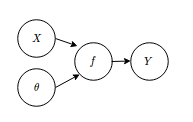
\includegraphics{q10.png}
\[p(\boldsymbol{Y}, \boldsymbol{X}, f, \boldsymbol{\theta}) = p(\boldsymbol{X}) p(\boldsymbol{\theta}) p(f|\boldsymbol{X},\boldsymbol{\theta})p(\boldsymbol{Y}|f)\]
Assumptions: - All X's are independent, shown by the
\(k(\pmb X, \pmb X)\)

    \subsubsection*{11}\label{section}

Marginalisation is a way to remove a variable that we aren't interested
in, such that the information we need from them isn't lost. We take the
liklihood function and multiply it by
\(p(f|\boldsymbol{X},\boldsymbol{\theta})\) and integrate it with
respect to \(f\). This allows us to look at the set of all functions,
and find an \(f\) that maximises the marginal likelihood. We don't know
what \(f\) is chosen however this isn't important to us.

This connects the prior to the data by removing the intermediate
paramater \(f\) that was a function of the other 2 parameters. Instead
of the data \(\boldsymbol(Y)\) relying on only some \(f\), it now relies
upon just the data \(X\) and some parameter \(\boldsymbol{\theta}\).

\(\boldsymbol{\theta}\) remaining implies that \(\boldsymbol{Y}\) is
dependent on both the input data (X) as well as \(\boldsymbol{\theta}\)
and that different \(\boldsymbol{\theta}\) values will result in a
different \(f\) that will give the maximum marginal liklihood.

    \subsubsection*{12}\label{section}

On the left is the visualisation of the prior/posterior and on the right
you can see a sample of functions from the prior/posterior.\\
Adding the first data point we see that the posterior shifts and becomes
smaller and the functions seem to pass through the general area of the
data point. On adding more data points the posterior starts to converge
on the parameters and the functions move closer together and are very
closely aligned to the direction of the data points.
    \begin{center}
    \adjustimage{max size={0.9\linewidth}{0.9\paperheight}}{output_14_0.png}
    \end{center}
    { \hspace*{\fill} \\}

    \begin{center}
    \adjustimage{max size={0.9\linewidth}{0.9\paperheight}}{output_14_1.png}
    \end{center}
    { \hspace*{\fill} \\}

    \begin{center}
    \adjustimage{max size={0.9\linewidth}{0.9\paperheight}}{output_14_2.png}
    \end{center}
    { \hspace*{\fill} \\}

    \begin{center}
    \adjustimage{max size={0.9\linewidth}{0.9\paperheight}}{output_14_3.png}
    \end{center}
    { \hspace*{\fill} \\}

    \subsubsection*{13}\label{section}

The first plot has value of length scale equal to 1 while the second one
has length scale equal to 2.\\
The length scale is directly proportional to the covariance of the
Gaussian Process and we see that decreasing the value makes the
functions noisier as the covariance decreases.

The length scale encodes the assumption of smoothness of the function.
    \begin{center}
    \adjustimage{max size={0.9\linewidth}{0.9\paperheight}}{output_16_0.png}
    \end{center}
    { \hspace*{\fill} \\}

    \begin{center}
    \adjustimage{max size={0.9\linewidth}{0.9\paperheight}}{output_16_1.png}
    \end{center}
    { \hspace*{\fill} \\}

    \subsubsection*{14}\label{section}

We can see that the samples from the posterior are less varied near the
data points and as we move away from the data points the uncertainity
increases and the function starts to resemble the prior. This is
desirable since it means that where we see data the model fits to the
data and where no data is present it is represented by our prior belief
but also has a high uncertainity.
    \begin{center}
    \adjustimage{max size={0.9\linewidth}{0.9\paperheight}}{output_18_0.png}
    \end{center}
    { \hspace*{\fill} \\}

    \subsubsection*{15}\label{section}

The difference between a preference and an assumption is merely
contextual. The overarching idea behind them is the same, however
depending on the situation or context of the model you are creating, the
decision is made as to whether preference or assumption is the preferred
term. Both of these terms allow is to improve on our prior in some way,
whether it be that we are "assuming" something about our input data, or
we actually have some kind of "preference" to what form it takes.

    \subsubsection*{16}\label{section}

The assumption we have encoded with this prior is that all the
parameters are equally important, shown by the identity matrix as a
covariance matrix. Since there is no covariance between the separate
parameters, we are showing they're all equally important and independent
of each other.

    \subsubsection*{17}\label{section}

We know \(y = Wx + \mu + \epsilon\)

And the marginal distribution is a gaussian given by

\(p(y) = \mathcal{N}(y\)\textbar{}\(\mu, C)\)

To derive the mean and covariance we get:

\(\mathbb E[y] = \mathbb E[\pmb W\pmb X + \mu + \epsilon] = \mu\)

\(cov[y] = \mathbb E[(\pmb W\pmb X + \epsilon)(\pmb W\pmb X + \epsilon)^T] = \mathbb E[\pmb W\pmb X\pmb X^T\pmb W^T] + \mathbb E[\epsilon.\epsilon^T] = \pmb W\pmb W^T + \sigma^2\pmb I\)

This covariance shows that it's entirely in terms of W and no X, so we
have removed X.

    \subsubsection*{18}\label{section}

\begin{enumerate}
\def\labelenumi{\alph{enumi})}
\item
  MAP and ML are different in that MAP maximises the posterior, whilst
  ML maximises the likelihood. However, if the prior of the distribution
  is a constant, MAP and ML are actually the same. Unlike MAP, ML does
  not weight it's data (shown by the exclusion of the prior) and
  therefore doesn't generate an estimate of the uncertainty of it's
  results. Type 2 ML marginalises out parts that we don't really need.
\item
  As we observe more data, you can update your posterior further and
  further, whilst throughout the likelihood does not particularly
  change. Visually, the posterior distribution homes in on the "correct
  answer", whilst the likelihood remains basically the same.
\item
  The two expressions are equal, as the denominator on the left hand
  side marginalises out W, and since we are maximising in terms of W,
  having a term without W is simply a constant, and so makes no
  different to our numerator.
\end{enumerate}

    \subsubsection*{19}\label{section}

% \begin{enumerate}
% \def\labelenumi{\alph{enumi})}
% \item
%   \(\mathcal{L}(\pmb W) = constant + log\)\textbar{}\(\pmb C(\pmb W)\)\textbar{}\
%   + \sum\_\{i\}\^{}\{N\}
%   (y\_i)\textsuperscript{T(\pmb C(\pmb W))}\{-1\}y\_i\$
% \item
%   \(\frac{\delta}{\delta\pmb W_{ij}}\log\)\textbar{}\(\pmb C\)\textbar{}\$
%   = tr (\pmb C\^{}\{-1\}\frac{\delta\pmb C}{\delta\pmb W_{ij}})\$
% \end{enumerate}

\(tr ( \pmb Y\pmb Y^T \frac{\delta\pmb C^{-1}}{\delta\pmb W_{ij}}) = tr ( \pmb Y\pmb Y^T (-\pmb C^{-1} \frac{\delta\pmb C}{\delta\pmb W_{ij}}\pmb C^{-1}))\)

    \subsubsection*{20}\label{section}

Generally it's more simple to marginalise out \(f\) since a function can
easily be incorporated into the model itself, if we still have the
variables that parametrize that function included in the model. Since
\(f\) only depends upon these parameters, it is therefore simple to
marginalise. \(\boldsymbol{X}\) however can be much larger since it's
the input data itself and should have some effect on the output
\(\boldsymbol{Y}\). To marginalise \(\boldsymbol{X}\) the model would
have to change every time for a new input which makes the process a lot
more complex. It also doesn't remove the uncertainty introduced by an
intermediate function such as \(f\).

    \subsubsection*{21}\label{section}

Our data was generated by first passing the x through a non-linear
function and then passing that output through a linear function. The
linear function generates data that is 10 dimensional. This data cannot
be visualised since it is in a higher dimension than we can visualise.
Hence we need to learn a mapping from this higher dimensional space to
one that we can visualise. Using our linear functions we can only learn
the linear mapping of the data which means that what we are left with is
the non-linear part of the Y which is a spiral since the non-linear part
is described by {[}xsin(x), xcos(x){]}
    \begin{center}
    \adjustimage{max size={0.9\linewidth}{0.9\paperheight}}{output_26_2.png}
    \end{center}
    { \hspace*{\fill} \\}

    \subsubsection*{22}\label{section}

It is the simplest possible model since it places a uniform probability
mass over the entire space which is mathematically very nice.

It is the most complex model since it places a uniform probability mass
over the entire space and so tries to spread the probability mass over
the entire dataset space which could lead to the model being penalised
by Bayes' Rule.

    \subsubsection*{25}\label{section}

We see that the sum of the evidence over the entire dataspace for every
model is about 1. This is the expected outcome since we are essentially
integrating our probability distribution to get the area under the curve
which should sum to one.
    \subsubsection*{26 and 27}\label{and-27}
    \begin{center}
    \adjustimage{max size={0.9\linewidth}{0.9\paperheight}}{output_31_0.png}
    \end{center}
    { \hspace*{\fill} \\}

    \begin{center}
    \adjustimage{max size={0.9\linewidth}{0.9\paperheight}}{output_31_2.png}
    \end{center}
    { \hspace*{\fill} \\}

    \begin{center}
    \adjustimage{max size={0.9\linewidth}{0.9\paperheight}}{output_31_4.png}
    \end{center}
    { \hspace*{\fill} \\}

    \begin{center}
    \adjustimage{max size={0.9\linewidth}{0.9\paperheight}}{output_31_6.png}
    \end{center}
    { \hspace*{\fill} \\}

    \begin{center}
    \adjustimage{max size={0.9\linewidth}{0.9\paperheight}}{output_31_8.png}
    \end{center}
    { \hspace*{\fill} \\}

    \subsubsection{30}\label{section}

Throughout this assignment, we have created and understood parametric
and non-parametric models. We have learned the differences and uses of
different model types and gaussian processes, as well as deriving and
performing marginalisations amongst other things. We feel the purpose of
performing this assignment has been to give as a "hands-on" approach to
machine learning, and provide a clearer picture of what everything does.


    % Add a bibliography block to the postdoc



    \end{document}
